\subsection{Data Set}
Over a span of three days, data was collected using the methods outlined in Section \ref{sec:data_methods}. A total runtime of \SI{5.78}{h} was collected. The robot traveled \SI{472}{m} and broke down four times. 

\subsubsection{Distributions}
Presented in this section is both the task space and joint space distributions of the dataset. In task space, the position, velocity, and acceleration of the end effector are displayed in the histogram in Figure \ref{fig:dataset_dist_task}. In joint space, the motor current is displayed along with the motor current's first and second derivatives in Figure \ref{fig:dataset_dist_joint}. 

\begin{figure}[h]
    \centering
    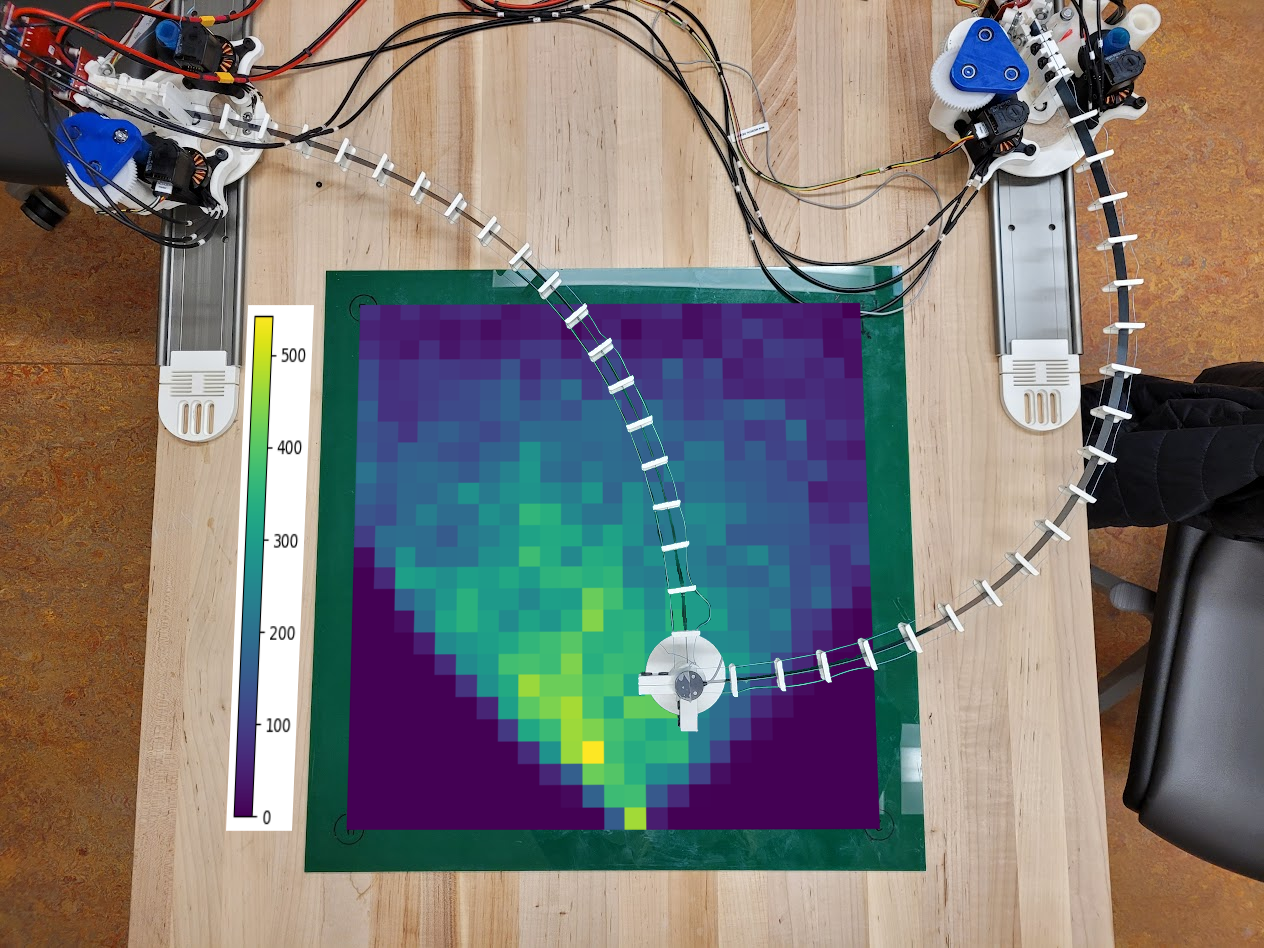
\includegraphics[width=\textwidth]{images/dataset_overlay.png}
    \caption{Data set position distribution overlaid on robot workspace}
    \label{fig:dataset_overlay}
\end{figure}

Figure \ref{fig:dataset_overlay} shows the task space position distribution overlaid on the robot's workspace. The densest distribution point at the middle-bottom of the workspace corresponds with the robot's home position. This is where the robot starts each time it is powered on and where it returns to in recovery mode. 

\begin{figure}[h]
     \centering
     \begin{subfigure}[b]{0.48\textwidth}
         \centering
         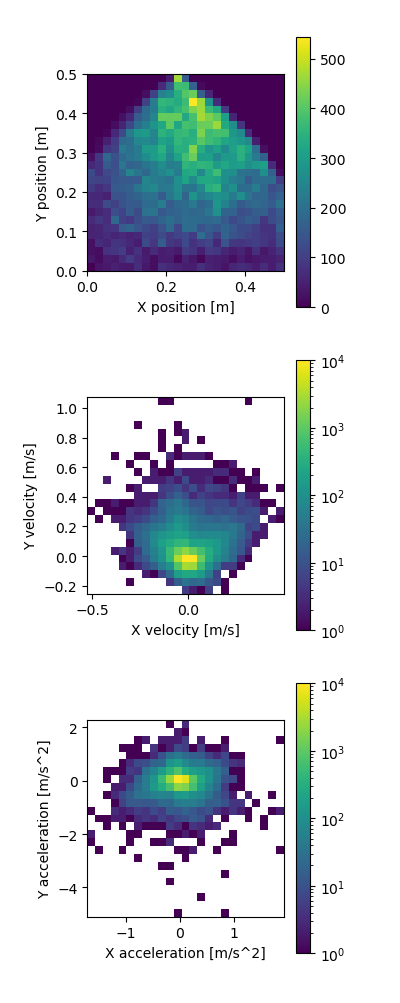
\includegraphics[width=\textwidth]{images/dataset_distribution.png}
         \caption{Task space distribution}
         \label{fig:dataset_dist_task}
     \end{subfigure}
     \hfill
     \begin{subfigure}[b]{0.48\textwidth}
         \centering
         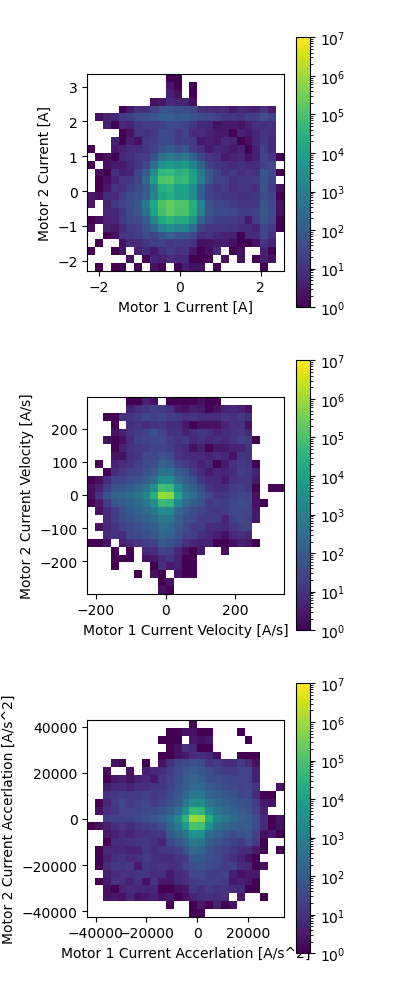
\includegraphics[width=\textwidth]{images/dataset_distribution_joint.png}
         \caption{Joint space distribution}
         \label{fig:dataset_dist_joint}
     \end{subfigure}
        \caption{Data set distribution histograms}
        \label{fig:dataset_dist}
\end{figure}

Table \ref{tab:dataset_runtype} breaks down the sample termination cases for the dataset, along with relevant metrics for each. Note that all cases that ended in an error termination were manually removed due to data corruption. 

\begin{table}[h]
    \centering
    \caption{Data set run type summary}
    \makebox[\textwidth][c]{\begin{tabular}{p{0.15\linewidth} | p{0.12\linewidth} | p{0.12\linewidth} | p{0.12\linewidth} | p{0.14\linewidth} | p{0.12\linewidth} | p{0.1\linewidth}}
        \textbf{Data Run Type} & \textbf{Average Distance [m]} & \textbf{Average Velocity [m/s]}  & \textbf{Average Duration [s]}  & \textbf{Total Distance [m]} & \textbf{Total Duration [s]} & \textbf{Total Runs}\\
        \hline
        Success & 0.1038 & 0.0294 & 4.49 & 367.78 & 15,915 & 3543\\
        \hline
        Stalled & 0.1142 & 0.0184 & 6.55 & 73.29 & 4,203 & 642\\
        \hline
        Aurora Lost & 0.1281 & 0.0338 & 3.65 & 1.79 & 51 & 14\\
        \hline
        Recovery & 0.3962 & 0.0591 & 6.69 & 22.77 & 401 & 60\\
        \hline
        Mode Switched & 0.1157 & 0.0322 & 4.66 & 5.44 & 219 & 47\\
        \hline
        User Terminated & 0.0811 & 0.0217 & 3.42 & 0.16 & 7 & 2\\ 
    \end{tabular}}
    \label{tab:dataset_runtype}
\end{table}